\documentclass{amsart}
\usepackage{amsmath}
\usepackage{amssymb}
\usepackage{graphicx}
\newcommand{\me}{
    \author{Abhay Shankar K: cs21btech11001}
    \maketitle
}
\begin{document}
\title{Assignment 4}
\me

\section{Overview}
\begin{itemize}
    \item There are m passenger threads and n car threads, and each thread waits on the availability of a thread of the other kind.
    \item A counting sempahore is used for the passenger wait, whereas the car threads busy-wait.
    \item When each thread finishes operation, it appends all the benchmarking data onto a global vector, 
    and once all threads finish, this data is averaged and written to a csv file.
    \item The enclosed python scripts read from this file and generate graphs. Building the enclosed latex file generates the pdf report.
\end{itemize}

\section{Contents}
\subsection{Classes}
\begin{itemize}
    \item Params: Contains all the user-defined parameters, taken from \texttt{inp-params.txt}
    \item Fleet: Represents the collection of cars in the park. \begin{itemize}
        \item \texttt{acquire()}: `Polls' the car threads by iterating through the \texttt{status} deque. When a car is \texttt{Waiting}, changes it's state to \texttt{Service} atomically and returns the index.
        \item \texttt{release()}: Takes the index of a car thread and sets it's status to \texttt{Cooldown}
        \item \texttt{ready()}: Sets status to \texttt{Waiting}.
        \item The Constructor and Destructor spawn and join threads respectively. Furthermore, the Constructor opens the \texttt{glob} semaphore and the Destructor closes it.
    \end{itemize}
    \item Crowd: Represents the collection of passengers in the park. \begin{itemize}
        \item \texttt{leave()}: Decrements atomic variable indicating \# passengers in museum.
        \item \texttt{alive()}: Returns whether any passengers left. Used for Car thread termination.
        \item The Constructor and Destructor spawn and join threads respectively.
    \end{itemize}
    \item Time: Used for calculating the average ride time (as required by the question). \begin{itemize}
        \item \texttt{exit()}: Records end of passenger thread.
        \item \texttt{power\_off()}: Records end of car thread.
        \item \texttt{out()}: Writes average ride time to file.
        \item The Constructor reserves space for the \texttt{vector<chrono::duration<double>>} and opens two semaphores. The Destructor unlinks the semaphores.
    \end{itemize}
    \item CarStatus: Enum representing the three states of a car.
\end{itemize}

\subsection{Functions}
\begin{itemize}
    \item \texttt{cars\_init()}: Starting point for Car threads. Mostly passive, resulting in scheduling abnormalities causing a sporadic segmentation fault (fixed). Logs readiness to file, busy waits until status changes to \texttt{Service}, then logs occupancy to file, busy waits until status changes to \texttt{Cooldown}, then sleeps. Repeat while any passenger thread is active.
    \item \texttt{passengers\_init()}: Starting point for Passenger threads. For k iterations, \begin{itemize}
        \item Wander: sleep for a random duration.
        \item Perform request and acquire a Car.
        \item Yield - fix to the aforementioned segfault.
        \item Ride: sleep for a random duration.
        \item Release the Car.
    \end{itemize}
    with appropriate IO as mentioned in the question statement.
    \item \texttt{now()}: Returns current system time.
\end{itemize}

\section{Graphs}
\subsection{Vary Passengers}.

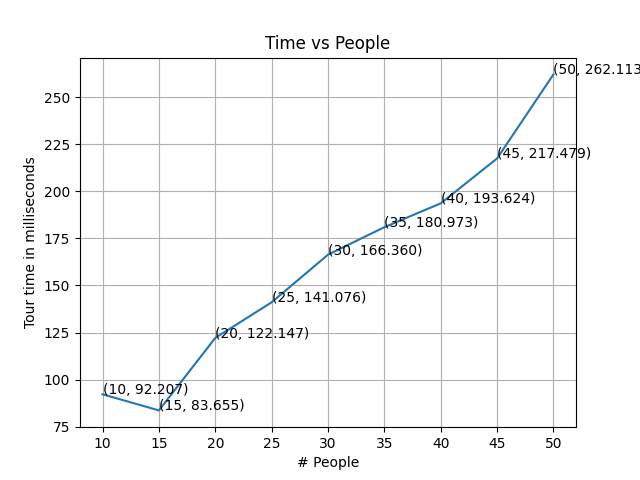
\includegraphics[scale = 0.9]{../people.png}

The graph is as one would expect, with a clear linear increase in time as the number of passengers increase due to contention for cars as well as for the cores.

Due to the compounding effects of contention, the slope of the graph increases slightly for higher \# threads.

\subsection{Vary Cars}.

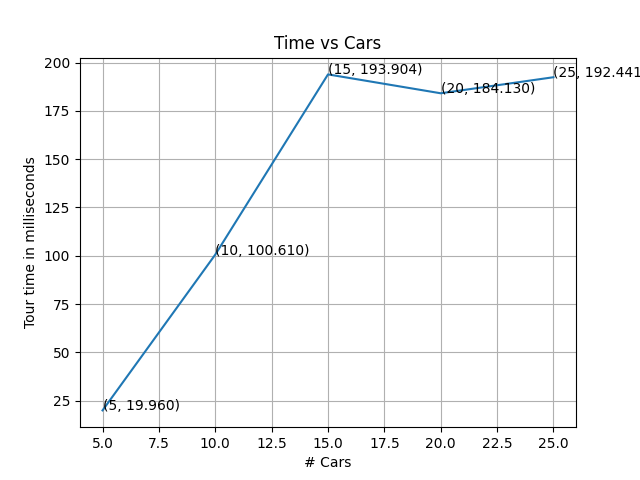
\includegraphics[scale = 0.9]{../cars.png}

The graph is somewhat atypical, because while an increase in \# car threads would decrease contention among passengers for cars, it increases contention among threads for cores, and clearly the latter effect dominates for small \# threads - the time taken increases linearly - but balances out for larger \# threads.

In earlier versions, this was not the case, and tour time showed a marked decline with increase in \# cars. However, the \texttt{yield} call - required to prevent starvation and subsequent segmentation faults - in \texttt{passenger\_init()} reduced passenger contention, and thus we have this graph.
\end{document}